\documentclass{article}

\usepackage{graphicx}

\title{Yelp and Crime Data}  % TODO
\author{Kenneth Lin, Tom McCormick, Sid Naik}
\date{\today}

\begin{document}
\maketitle

\section{Introduction}

For our CS 194 final project, we decided to investigate the potential
relationship between the City of San Francisco public safety data set and
the data set provided by the Yelp API. At first, we explored each data set
individually to discover general patterns in the data set. After that was
completed, we looked at the nearest 20 restaurants near each crime to see
if we could discover any common patterns of restaurants close to crimes.
% TODO conclusions

\section{City of San Francisco Public Safety Data Set}

\begin{center}
  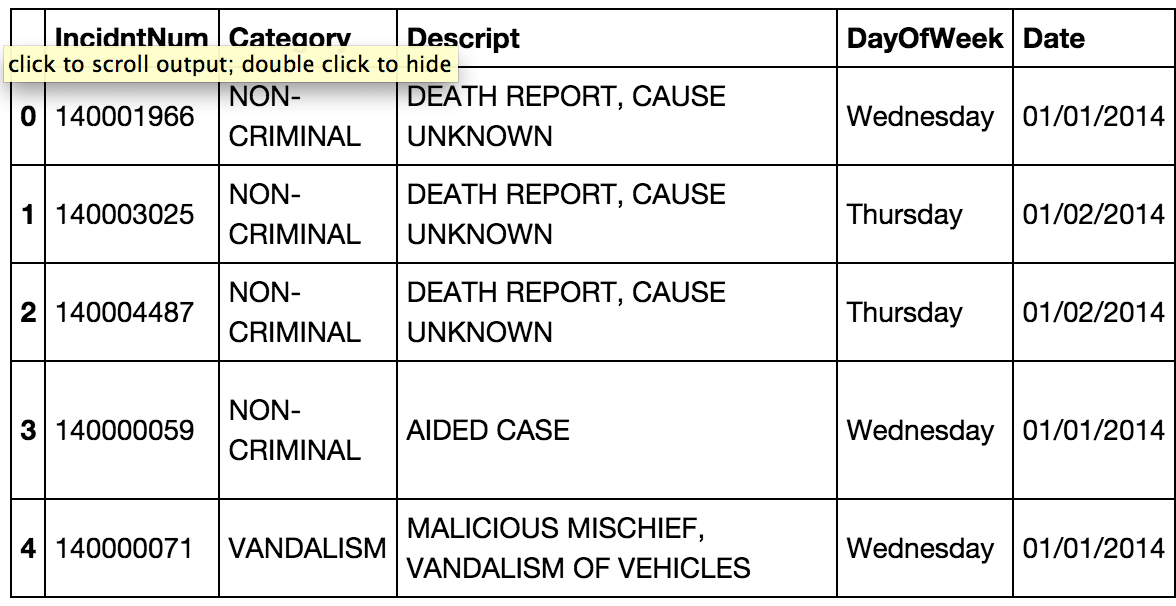
\includegraphics[scale=0.5]{sf_city_sample_1.png} \\
  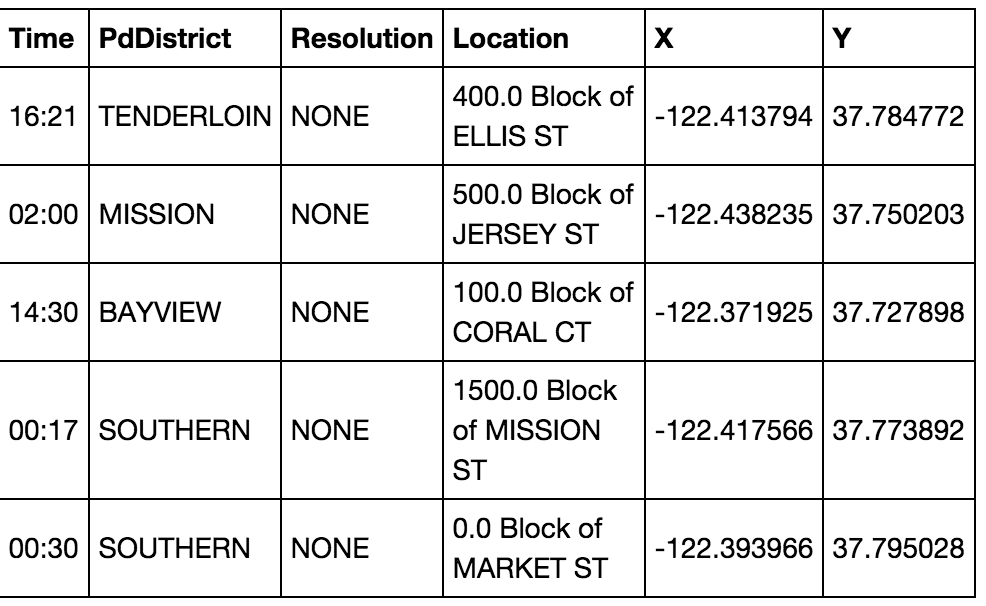
\includegraphics[scale=0.5]{sf_city_sample_2.png} \\
  Figure 1: Sample of San Francisco crime data set
\end{center}

The majority of the fields are self-explanatory. However, there are a few
things to note:
\begin{enumerate}
\item Category and descript are both categories, but category is more
  general. There are only 36 different ``Categories'' while there are 499
  different ``Descript''s in the year of 2014.
\item Resolution, though none are shown in the sample above, denote whether
  any action was taken and what that action was.
\item X denotes longitude, while Y denote latitude.
\end{enumerate}

A more detailed analysis is in the attached \texttt{analysis.ipynb}.

\section{Yelp Data Set}

\end{document}
